% !TeX program = xelatex
\documentclass[12pt,a4paper]{article}
\usepackage{fontspec}
\setmainfont{Times New Roman}
\setsansfont{Arial}
\setmonofont{Courier New}
\usepackage[english,russian]{babel}
\usepackage{amsmath,amssymb}
\usepackage[margin=22mm]{geometry}
\usepackage{graphicx,float}
\usepackage[unicode,hidelinks]{hyperref}
\selectlanguage{russian}
\setlength{\emergencystretch}{3em}
\setlength{\parindent}{1.25cm}
\newcommand{\topic}[1]{\par\medskip\noindent\textbf{#1}\par\nobreak\smallskip}
\renewcommand{\thefootnote}{\arabic{footnote})}
\title{Вопрос 1. Основные физические сведения о пористых средах}
\author{Н. Е. Леонтьев\\\large Основы теории фильтрации}
\date{Учебное пособие. 2-е издание. Москва: МАКС Пресс, 2017\\Глава I, §§ 1--2. Печатные страницы 7--13}
\begin{document}
\maketitle
\noindent\textit{Перенос выбранного фрагмента оригинала в редактируемый LaTeX. Страницы файла: 7--13; на странице 13 текст заканчивается перед § 3. Нумерация формул и рисунков сохранена; размещение материала перевёрстано.}
% Источник: Leontiev-2017.pdf; печатная страница: 7; страница файла: 7
\section*{Глава I. Основные понятия и уравнения теории фильтрации}
\label{q1:chapter-i}
\subsection*{§ 1. Описание фильтрации в рамках механики сплошных сред}
\label{q1:section-1}
\setcounter{footnote}{0}
\topic{Фильтрация}
\textit{Фильтрацией} называется движение (просачивание) жидкостей и газов через пористые среды под действием каких-либо факторов\footnote{Термин «фильтрация» также употребляется в более узком смысле как название процесса очищения жидкости или газа от примесей при течении через фильтр. В англоязычной литературе при описании этих процессов употребляется термин \textit{filtration}, в то время как о фильтрации в широком смысле этого слова говорят обычно как о «течении жидкости через пористую среду» (\textit{flow of a fluid through a porous medium}).}. Фильтрационные процессы широко распространены и встречаются как в повседневной жизни (движение табачного дыма в сигарете, очистка водопроводной воды в бытовом фильтре, смачивание губки для мытья посуды), так и в явлениях, влияющих на благосостояние целых государств (передвижение нефти и природного газа в подземных пластах, миграция влаги в плодородных почвах, работа технологических устройств химических предприятий).

\topic{Описание фильтрации в рамках МСС}
Вне зависимости от вызывающих фильтрацию причин, которые могут быть совершенно различными --- например, перепад давлений на границе среды, действие внешних массовых сил (сила тяжести, силы инерции, электромагнитные силы) или капиллярных сил на межфазных границах, деформация пористой среды и др.,--- речь всегда идет о движении жидкости по сложной системе разветвленных каналов, сообщающихся между собой. Как правило, внутренняя поверхность порового пространства имеет случайную структуру и не бывает точно известна, поэтому прямое описание движения жидкости во всех подробностях оказывается невозможным. Но и даже если бы мы каким-либо образом полностью узнали внутреннюю геометрию пор, то и в этом случае практическое нахождение параметров течения в порах на основе уравнений гидродинамики все равно было бы возможным лишь в небольшом числе частных случаев (например, для искусственно созданной периодической среды).

К счастью, однако, в большинстве приложений характерные линейные размеры рассматриваемых фильтрационных задач
% Источник: Leontiev-2017.pdf; печатная страница: 8; страница файла: 8
много больше характерного размера пор, а при практическом изучении фильтрационных явлений обычно интересуются осредненными характеристиками течения. Это позволяет при описании крупномасштабных явлений рассматривать пористый материал как сплошную среду, характеристики которой (плотность и давление жидкости в порах и др.) в каждой точке получаются в результате осреднения по некоторой окрестности, содержащей достаточно большое число пор\setcounter{footnote}{0}\footnote{Этот переход вполне аналогичен переходу от молекулярно-кинетической теории к континуальному описанию в случае, когда характерный размер явления много больше длины свободного пробега отдельной молекулы, с той лишь разницей, что в случае фильтрационных явлений описание течений на микроуровне тоже может быть осуществлено в рамках механики сплошных сред.}.

\begin{figure}[H]
\centering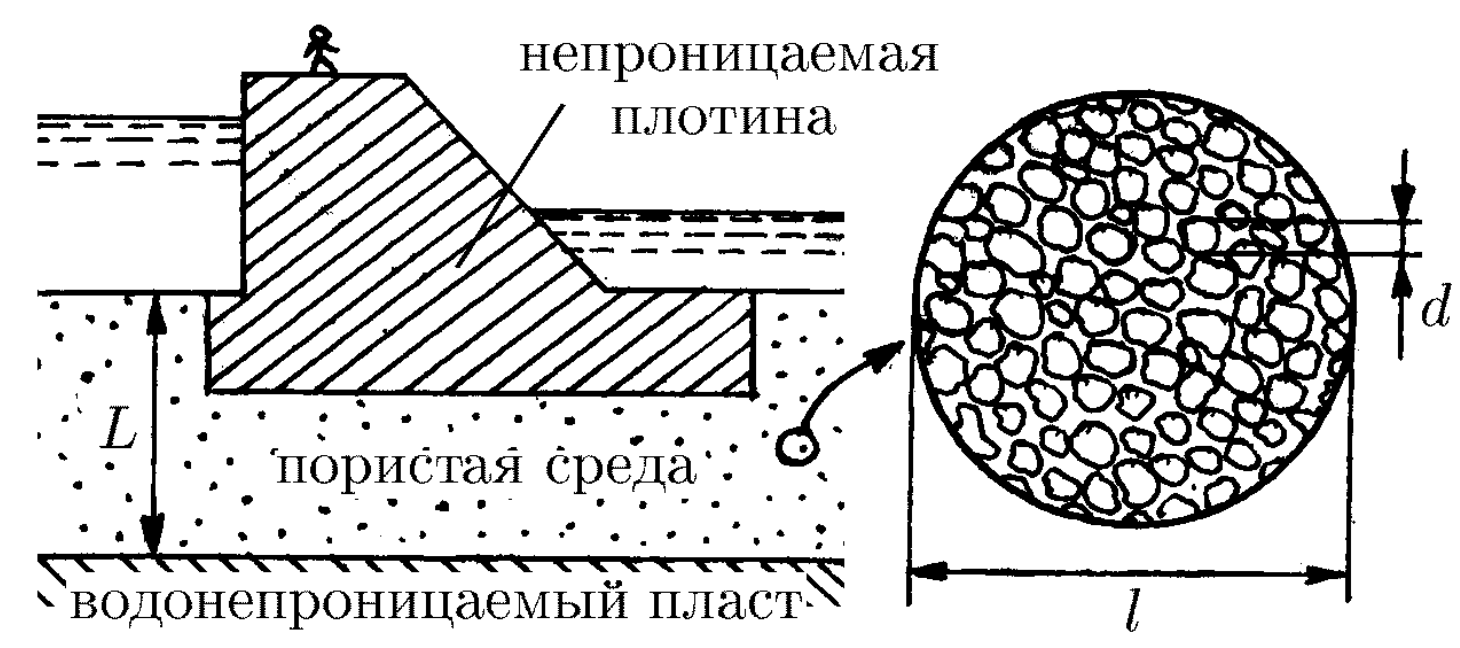
\includegraphics[width=.82\linewidth]{figures/figure-1.png}
\caption{}\label{q1:fig-1}
\end{figure}
Например, при просачивании воды через пористый пласт под непроницаемой бетонной плотиной (рис.~\ref{q1:fig-1}) характерный размер пор $d$ (доли миллиметра) много меньше характерного размера пористого пласта $L$ (десятки метров), поэтому мы можем перейти от описания течения на микроуровне (течение внутри конкретной поры) к описанию на макроуровне, считая, что, например, среднее давление $p$ жидкости в порах (в некотором месте внутри пласта в какой-то момент времени) получается осреднением давления в поровом пространстве внутри достаточно малого объема, размеры $l$ которого будут, с одной стороны, много меньше $L$ и, с другой стороны, много больше $d$ (скажем, порядка десятков сантиметров):
\begin{equation}
d\ll l\ll L.
\tag{1.1}\label{q1:eq-1-1}
\end{equation}
При этом, естественно, рассматриваемая величина (в нашем примере давление) будет, вообще говоря, некоторой функцией от
% Источник: Leontiev-2017.pdf; печатная страница: 9; страница файла: 9
координат и времени: $p=p(x,y,z,t)$.

\subsection*{§ 2. Параметры, описывающие накопление и перенос жидкости в пористой среде}
\label{q1:section-2}
\topic{Пористость}
Важной характеристикой пористой среды является \textit{пористость} (или \textit{порозность}) $m$, равная относительной объемной доле порового пространства в материале. Пористость определяет количество жидкости, которое может содержаться в некотором объеме пористой среды (если жидкость целиком заполняет внутрипоровое пространство). Если для образца однородного пористого материала объемом $V$ объем пор составляет $V_{\text{п}}$, то пористость этого образца $m=V_{\text{п}}/V$.

Пористость, очевидно, является безразмерной величиной, значения которой лежат в интервале $0<m<1$. Для ориентировки укажем, что пористость почв лежит в диапазоне $0{,}3$--$0{,}7$, речного песка --- $0{,}3$--$0{,}55$, нефтегазоносных пластов, встречающихся на практике, --- $0{,}1$--$0{,}2$.

У некоторых пористых материалов часть пор изолирована от остального связного порового пространства или заполнена другой средой (например, при фильтрации воздуха в почве часть пор занята водой, удерживаемой в поровом пространстве за счет капиллярных сил). В подобной ситуации эти поры не участвуют в накоплении и перемещении интересующей нас жидкости внутри пористой среды, и поэтому вместо введенной выше величины (ее называют \textit{полной} или \textit{общей пористостью}) удобно использовать \textit{активную (эффективную) пористость}, равную объемной доле связанных между собой пор, которые могут быть заполнены жидкостью извне. В качестве примера сред с различными полной и активной пористостями можно привести кору пробкового дерева или пористый шоколад, у которых полная пористость отлична от нуля --- в этих материалах есть поры, в то время как их активная пористость равна нулю --- через них жидкость фильтроваться не может.

Для неоднородных пористых сред, свойства которых могут меняться от точки к точке, пористость $m$ будет некоторой функцией пространственных координат. Если пористая среда может деформироваться (это происходит, например, при утрамбовке грунта или изменении давления в жидкости в порах), то величина пористости может меняться и со временем: $m=m(x,y,z,t)$.

% Источник: Leontiev-2017.pdf; печатная страница: 10; страница файла: 10
\begin{figure}[H]
\centering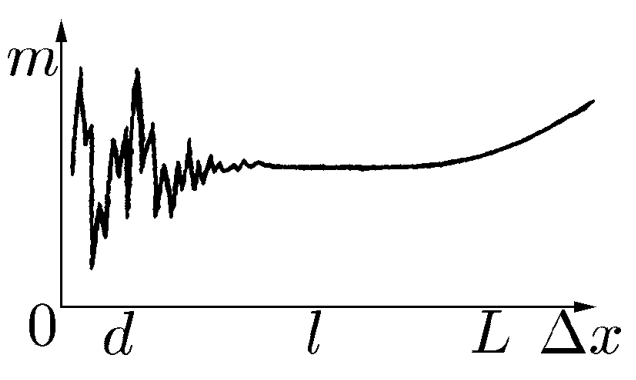
\includegraphics[width=.36\linewidth]{figures/figure-2.png}
\caption{}\label{q1:fig-2}
\end{figure}
Подчеркнем, что при континуальном описании величина пористости (так же как и значения всех остальных осредненных параметров) определяется с помощью осреднения по области с размером порядка $l$, удовлетворяющим \eqref{q1:eq-1-1}. Если бы осреднение проводилось по маленькой области с размером $\Delta x\sim d$, то значение $m$, вычисленное по формуле $m=V_{\text{п}}/V$, испытывало бы существенные колебания с увеличением $\Delta x$ (качественный вид этой зависимости показан на рис.~\ref{q1:fig-2}).

\topic{О введении характерного размера пор}
\setcounter{footnote}{0}
По поводу уже упоминавшегося понятия характерного размера пор $d$ сделаем следующее замечание. В реально встречающихся пористых средах размеры неоднородностей (размеры пор, размеры зерен) распределены случайным образом, причем часто бывают ситуации, когда плотность распределения пор по радиусам имеет даже несколько максимумов. Поэтому, строго говоря, введение характерного размера может быть произведено \textit{неоднозначно}\footnote{В качестве характерного размера можно, например, взять величину, пропорциональную отношению объема пористого образца к площади поверхности порового пространства, или размер, соответствующий какой-либо характерной точке (медиане, точке максимума) на графике плотности распределения пор по радиусам.}, однако определение такой величины бывает удобно для проведения оценок по порядку при анализе уравнений.

\topic{Просветность}
Если сделать мысленный поперечный разрез образца пористой среды, то в образовавшемся сечении (обозначим его площадь $S$) часть площади $S_{\text{п}}$ будет приходиться на поры, а оставшаяся часть $S-S_{\text{п}}$ --- на твердое вещество пористой среды\footnote{«Каркас» пористой среды часто называют \textit{пористым скелетом} или \textit{матрицей}. Отметим также, что в отношении фильтрующейся среды (жидкой или газообразной) иногда применяется термин \textit{флюид}.}. Отношение $n$ площади пор в сечении к общей площади сечения называется \textit{просветностью (поверхностной пористостью)}: $n=S_{\text{п}}/S$.

Величина просветности зависит от того, через какую точку и в каком направлении проводится разрез среды, однако, что замечательно, \textit{среднее значение просветности} для большого набора параллельных сечений какого-то фиксированного образца равно
% Источник: Leontiev-2017.pdf; печатная страница: 11; страница файла: 11
пористости этого образца. В самом деле, возьмем цилиндрический образец пористой среды с площадью основания $S$ и высотой $h$ (рис.~\ref{q1:fig-3}) и осредним по высоте просветности $n(x)$ в поперечных сечениях образца (ось $x$ направлена вдоль образующей цилиндра). В результате для среднего значения просветности получим
\begin{equation*}
\begin{aligned}
\langle n\rangle&=\frac{1}{h}\int_0^h n(x)\,dx
=\frac{1}{Sh}\int_0^h Sn(x)\,dx=\\
&=\frac{1}{Sh}\int_0^h S_{\text{п}}(x)\,dx
=\frac{V_{\text{п}}}{V}=m.
\end{aligned}
\end{equation*}
\begin{figure}[H]
\centering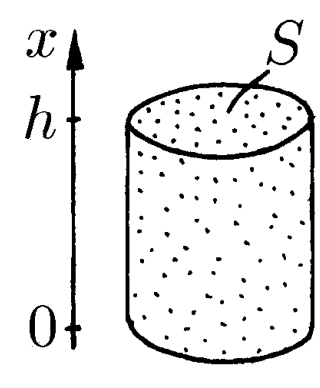
\includegraphics[width=.17\linewidth]{figures/figure-3.png}
\caption{}\label{q1:fig-3}
\end{figure}
\setcounter{footnote}{0}
Доказанное свойство позволяет приближенно считать пористость и просветность равными величинами для реальных пористых сред со случайной структурой: $m\approx n$. Отметим также, что эта особенность лежит в основе одного из методов измерения пористости\footnote{Проиллюстрируем идею метода на примере из повседневной жизни: для измерения пористости куска сыра нужно нарезать его тонкими ломтиками, для каждого ломтика подсчитать долю площади, приходящейся на дырки, и вычислить среднее значение полученных величин.} [7,18].

\topic{Об осредненных геометрических параметрах}
Обратим внимание, что упоминавшиеся выше геометрические по своей природе параметры (пористость, характерный размер пор, функция распределения пор по радиусам) в общем случае не характеризуют полностью способность пористой среды пропускать через себя жидкость. Например, проницаемую для жидкости пористую среду можно превратить в непроницаемую, если ввести внутри порового пространства некоторое количество тонких перегородок, которые практически не поменяют перечисленные средние характеристики, но существенно изменят проводимость среды.

\topic{Скорость фильтрации}
Для характеристики массопереноса при фильтрации жидкости (или газа) вводится векторная величина, называемая \textit{скоростью фильтрации}. Рассмотрим сначала простейший случай, когда жидкость движется вдоль тонкой прямолинейной трубки, заполненной пористым материалом. Для такого течения скорость фильтрации определяется как вектор $\boldsymbol{u}$, направленный в сторону движения
% Источник: Leontiev-2017.pdf; печатная страница: 12; страница файла: 12
жидкости, величина которого равна объемному расходу жидкости (объему жидкости, протекающей в единицу времени) в расчете на единицу площади \textit{полного поперечного сечения} трубки (включающего как поры, так и пористую среду).

Здесь важно подчеркнуть, что хотя скорость фильтрации имеет размерность скорости, она тем не менее не равна скорости движения отдельных частиц жидкости. Действительно, если $S$ --- площадь поперечного сечения трубки, $S_{\text{п}}$ --- часть площади этого сечения, приходящаяся на поры, то постоянство объемного расхода однородной несжимаемой жидкости можно записать в виде
\[
Q=|\boldsymbol{u}|S=vS_{\text{п}}=\mathrm{const},
\]
где $Q$ --- объемный расход жидкости через трубку, $v$ --- среднее значение проекции \textit{скорости частиц жидкости} на ось трубки, вычисленное по площади сечения, занимаемой порами. Отсюда получаем
\[
v=\frac{|\boldsymbol{u}|S}{S_{\text{п}}}=\frac{|\boldsymbol{u}|}{n}\approx\frac{|\boldsymbol{u}|}{m},
\]
т.е. средняя скорость частиц жидкости приблизительно в $1/m$ раз больше скорости фильтрации. Например, для речного песка с пористостью $m=0{,}3$ средняя скорость материальных частиц жидкости при их движении внутри пор превышает скорость фильтрации примерно в три раза.

В общем случае неодномерного движения жидкости в пористой среде \textit{скорость фильтрации} определяется как вектор $\boldsymbol{u}$, проекция которого на некоторое направление равна объемному расходу жидкости через единичную площадку, перпендикулярную данному направлению. С помощью этого определения легко вычисляются объемный расход $Q$ и массовый расход $Q_{\text{м}}$ жидкости через произвольную поверхность $\Sigma$, проведенную внутри пористой среды:
\begin{equation}
Q=\int_{\Sigma}\boldsymbol{u}\cdot\boldsymbol{n}\,d\sigma,
\qquad Q_{\text{м}}=\int_{\Sigma}\rho\boldsymbol{u}\cdot\boldsymbol{n}\,d\sigma,
\tag{2.1}\label{q1:eq-2-1}
\end{equation}
где $\rho=\rho(x,y,z,t)$ --- плотность фильтрующейся жидкости, $\boldsymbol{n}$ --- вектор нормали к поверхности $\Sigma$.

Удобство использования скорости фильтрации при практических исследованиях состоит в том, что с ее помощью можно находить расход жидкости без использования информации о пористости, которая явно не входит в соотношения \eqref{q1:eq-2-1}.

% Источник: Leontiev-2017.pdf; печатная страница: 13; страница файла: 13
Встречающиеся в гидрологической и нефтепромысловой практике скорости фильтрации как правило имеют достаточно малые значения (порядка метров в сутки), однако в некоторых природных процессах скорости фильтрации бывают сравнительно велики (например, при нестационарной фильтрации газа, вызванной резкими изменениями давления, в породах с узкими щелями между порами скорости фильтрации могут иметь порядок метров в секунду).

\topic{О моделировании структуры пористой среды}
Несмотря на то, что поровое пространство реальных сред имеет случайную структуру, качественные (а иногда и количественные) зависимости их фильтрационных свойств от средних геометрических параметров можно получить уже на элементарных геометрических моделях, которые благодаря своей простоте выявляют «физику» происходящих процессов.

Примерами таких моделей, для которых можно получить либо аналитическое, либо численное решение, служат пористая среда, составленная из параллельных цилиндрических капилляров с некоторым распределением радиусов (рис.~\ref{q1:fig-4}); среда, в которой происходит поперечное обтекание пучка параллельных цилиндров (модель течения в волокнистой среде); среда из периодически расположенных одинаковых частиц; разветвленная сеть цилиндрических капилляров и т.п.
\begin{figure}[H]
\centering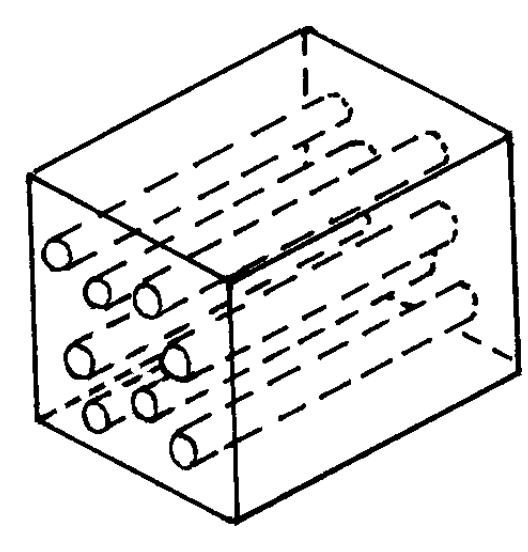
\includegraphics[width=.30\linewidth]{figures/figure-4.png}
\caption{}\label{q1:fig-4}
\end{figure}
% Конец § 2. Следующий заголовок оригинала: § 3. Законы сохранения массы и импульса при фильтрации в пористой среде.

\end{document}
